\section{Семинар 5. Принцип Дирихле и комбинаторные конфигурации}
\noeqref{eq:arith_prog_sum, eq:repunit_diff, eq:dirichlet_approx_thm}
\noeqref{eq:frac_part_def, eq:cube_ineq, eq:dio_final, eq:comb_paths}
\noeqref{eq:circ_perm, eq:necklace_count, eq:comb_no_rep_sem5}
\noeqref{eq:comb_rep_sem5, eq:eq_nat_sol}

\begin{remark}[Обзор темы]
    Первая часть пятого семинара посвящена нетривиальным применениям 
    принципа Дирихле в экстремальных комбинаторных задачах, теории чисел 
    (делимость репьюнитов) и геометрии чисел (теорема Дирихле о совместных 
    диофантовых приближениях). Во второй части семинара разбираются задачи 
    перечислительной комбинаторики: подсчёт траекторий на решётках, 
    циклические перестановки и ожерелья, строго возрастающие 
    последовательности и число решений линейных уравнений в целых числах.
\end{remark}

\subsection{Применение принципа Дирихле}

\begin{problem}[\textbf{Таблица $6 \times 6$ из элементов $\{0, 1, -1\}$}]
    Можно ли заполнить квадратную таблицу размера $6 \times 6$ числами из 
    множества $\{-1, 0, 1\}$ так, чтобы все суммы чисел по каждой строке, 
    каждому столбцу и обеим главным диагоналям были попарно различны?
\end{problem}

\begin{proof}[Решение]~\\
    \begin{quote}
        Докажем от противного с помощью принципа Дирихле, что заполнить 
        таблицу требуемым образом \textbf{невозможно}.

        \textbf{1. Подсчёт числа сумм («кроликов»):} 
        В квадратной таблице $6 \times 6$ имеется $6$ строк, $6$ столбцов и 
        $2$ главные диагонали. Всего рассматривается:
        \[
            m = 6 + 6 + 2 = 14 \text{ сумм.}
        \]

        \textbf{2. Подсчёт возможных значений сумм («ящиков»):} 
        Каждая линия (строка, столбец или диагональ) состоит ровно из $6$ 
        клеток, в каждой из которых стоит число из множества $\{-1, 0, 1\}$.
        \begin{itemize}
            \item Минимально возможная сумма достигается, когда во всех $6$ 
            клетках линии стоят числа $-1$: $S_{\min} = 6 \cdot (-1) = -6$.
            \item Максимально возможная сумма достигается, когда во всех $6$ 
            клетках линии стоят числа $1$: $S_{\max} = 6 \cdot 1 = 6$.
        \end{itemize}
        Поскольку сумма целых чисел является целым числом, значение суммы 
        вдоль любой линии принадлежит целочисленному отрезку 
        $[-6, 6] \cap \Z = \{-6, -5, \dots, 0, \dots, 5, 6\}$. Всего таких 
        возможных целых значений:
        \[
            n = 6 - (-6) + 1 = 13 \text{ значений.}
        \]

        \textbf{3. Применение принципа Дирихле:} 
        Имеется $m = 14$ сумм и только $n = 13$ возможных значений для них. 
        Так как $14 > 13$, по принципу Дирихле хотя бы две из $14$ сумм 
        обязательно совпадут.
        
        \textbf{Ответ:} Нет, нельзя.
    \end{quote}
\end{proof}

\begin{problem}[\textbf{Выбор одноцветных и разноцветных шаров}]
    В мешке лежат $10$ чёрных, $10$ синих и $10$ белых шаров. Какое 
    наименьшее количество шаров необходимо вытащить вслепую (не глядя), 
    чтобы среди вытянутых шаров гарантированно нашлись:
    \begin{enumerate}
        \item хотя бы $2$ шара \textbf{одного} цвета;
        \item хотя бы $2$ шара \textbf{разных} цветов?
    \end{enumerate}
\end{problem}

\begin{proof}[Решение]~\\
    \begin{quote}
        Применим принцип Дирихле и метод оценки наихудшего сценария.

        \textbf{1. Два шара одного цвета:} 
        Имеется $n = 3$ цвета («ящика»): чёрный, синий и белый. В 
        наихудшем случае первые $3$ вытянутых шара окажутся разных цветов 
        (по одному каждого цвета). По принципу Дирихле при выборе 
        $m = 3 + 1 = 4$ шаров ($4 > 3$) хотя бы в один из трёх цветовых 
        классов попадут не менее двух шаров. Значит, достаточно вытащить 
        \textbf{$4$ шара}.

        \textbf{2. Два шара разных цветов:} 
        Чтобы нарушить условие и вытягивать шары только одного цвета как 
        можно дольше, в наихудшем случае мы можем вытащить подряд все $10$ 
        шаров одного и того же цвета (например, все $10$ чёрных шаров). 
        Тогда $11$-й вытянутый шар гарантированно будет иметь другой цвет 
        (синий или белый), что даст пару шаров разных цветов. Значит, 
        необходимо вытащить \textbf{$11$ шаров}.
    \end{quote}
\end{proof}

\begin{problem}[\textbf{Задача о камнях и грузовиках}]
    На каменоломне добыли $36$ камней, массы которых образуют 
    арифметическую прогрессию с начальным членом $a_0 = 490\text{ кг}$ и 
    шагом $b = 5\text{ кг}$. Можно ли увезти все эти камни на $7$ 
    грузовиках грузоподъёмностью $3\text{ т}$ ($3000\text{ кг}$) каждый?
\end{problem}

\begin{proof}[Решение]~\\
    \begin{quote}
        Упорядочим $36$ камней по возрастанию массы: 
        $a_k = a_0 + k b = 490 + 5k\text{ кг}$, где индекс $k$ пробегает 
        значения $0, 1, \dots, 35$. Тогда самый лёгкий камень весит 
        $a_0 = 490\text{ кг}$, а самый тяжёлый --- 
        $a_{35} = 490 + 5 \cdot 35 = 665\text{ кг}$. Найдём суммарную массу 
        всех $36$ камней по формуле суммы арифметической прогрессии:
        \begin{equation} \label{eq:arith_prog_sum}
            S_{36} = \frac{a_0 + a_{35}}{2} \cdot 36 = 
            \frac{490 + 665}{2} \cdot 36 = 1155 \cdot 18 = 20\,790\text{ кг}. 
            \tag{1}
        \end{equation}
        Общая грузоподъёмность $7$ грузовиков составляет 
        $7 \cdot 3000 = 21\,000\text{ кг} > 20\,790\text{ кг}$, то есть по 
        суммарной массе перевезти камни потенциально возможно.

        Заметим, что в один грузовик ($3000\text{ кг}$) нельзя погрузить $7$ 
        или более камней, так как даже $7$ самых лёгких камней весят:
        \[
            490 + 495 + 500 + 505 + 510 + 515 + 520 = 3535\text{ кг} > 
            3000\text{ кг}.
        \]
        Следовательно, в каждый грузовик помещается \textbf{не более $6$ 
        камней}. Чтобы увезти $36$ камней на $7$ грузовиках, мы можем 
        загрузить в первые $5$ грузовиков по $6$ камней ($30$ камней), а 
        оставшиеся $6$ самых тяжёлых камней разделить по $3$ штуки между 
        $6$-м и $7$-м грузовиками:
        \begin{itemize}
            \item Рассмотрим первые $30$ камней с индексами 
            $k \in \{0, 1, \dots, 29\}$ (от $a_0 = 490\text{ кг}$ до 
            $a_{29} = 635\text{ кг}$). Разобьём их на $15$ пар с одинаковой 
            суммой, объединяя $k$-й и $(29 - k)$-й камни:
            \[
                a_k + a_{29-k} = (490 + 5k) + (635 - 5k) = 1125\text{ кг}.
            \]
            Погрузим в каждый из первых $5$ грузовиков по $3$ такие пары 
            ($6$ камней). Масса груза в каждом из этих $5$ грузовиков 
            составит $3 \cdot 1125 = 3375\text{ кг}$, что превышает 
            $3000\text{ кг}$! Значит, в грузовик по $6$ штук могут 
            поместиться только достаточно лёгкие камни.
            \item Проверим, сколько максимум камней вообще может лежать в 
            грузовиках с $6$ камнями. Средняя масса камня в грузовике из 
            $6$ камней не должна превышать $3000 / 6 = 500\text{ кг}$. Но 
            массу $\le 500\text{ кг}$ имеют только первые три камня 
            ($490, 495, 500\text{ кг}$)! Даже один грузовик, загруженный 
            $6$ самыми лёгкими камнями ($k = 0, \dots, 5$), весит:
            \[
                490 + 495 + 500 + 505 + 510 + 515 = 3015\text{ кг} > 
                3000\text{ кг}.
            \]
        \end{itemize}
        Таким образом, \textbf{ни в один грузовик не может поместиться $6$ 
        камней}: любые $6$ камней весят не менее $3015\text{ кг} > 3000\text{ кг}$. 
        Значит, в каждый из $7$ грузовиков можно положить не более $5$ 
        камней, а во все $7$ грузовиков поместится не более 
        $7 \cdot 5 = 35$ камней (по принципу Дирихле при распределении 
        $m = 36$ камней по $n = 7$ грузовикам хотя бы в одном грузовике 
        окажется $\ge \lceil 36/7 \rceil = 6$ камней, чей суммарный вес 
        превысит $3000\text{ кг}$).

        \textbf{Ответ:} Нет, увезти все $36$ камней на $7$ грузовиках нельзя.
    \end{quote}
\end{proof}

\begin{problem}[\textbf{Делимость чисел из одних единиц (репьюнитов)}]
    Доказать, что для любого натурального числа $d \in \N$, не делящегося 
    ни на $2$, ни на $5$ ($\operatorname{НОД}(d, 10) = 1$), существует 
    число, записываемое в десятичной системе счисления одними единицами 
    ($\underbrace{11\dots 1}_{n}$), которое нацело делится на $d$.
\end{problem}

\begin{proof}[Решение]~\\
    \begin{quote}
        Обозначим через $R_k = \underbrace{11\dots 1}_{k}$ число, состоящее 
        из $k$ единиц. Рассмотрим последовательность из $d + 1$ таких чисел:
        \[
            R_1 = 1, \quad R_2 = 11, \quad R_3 = 111, \quad \dots, \quad 
            R_{d+1} = \underbrace{11\dots 1}_{d+1}.
        \]
        При делении целого числа на $d$ возможны ровно $d$ различных 
        остатков: $\{0, 1, 2, \dots, d - 1\}$. Поскольку мы рассматриваем 
        $d + 1$ чисел («кроликов») и $d$ возможных остатков по модулю $d$ 
        («ящиков»), по принципу Дирихле среди чисел $R_1, \dots, R_{d+1}$ 
        обязательно найдутся два числа $R_i$ и $R_j$ (пусть $1 \le i < j \le d + 1$), 
        дающие одинаковый остаток при делении на $d$:
        \[
            R_j \equiv R_i \pmod{d} \implies (R_j - R_i) \vdots d.
        \]
        Запишем разность $R_j - R_i$ в десятичной системе счисления:
        \begin{equation} \label{eq:repunit_diff}
            R_j - R_i = \underbrace{11\dots 1}_{j} - \underbrace{11\dots 1}_{i} = 
            \underbrace{11\dots 1}_{j-i}\underbrace{00\dots 0}_{i} = 
            R_{j-i} \cdot 10^i. \tag{2}
        \end{equation}
        По доказанному произведение $R_{j-i} \cdot 10^i$ делится на $d$. 
        Но по условию число $d$ не делится ни на $2$, ни на $5$, то есть 
        взаимно просто со степенью десятки: $\operatorname{НОД}(d, 10^i) = 1$. 
        По лемме Евклида из делимости $(R_{j-i} \cdot 10^i) \vdots d$ и 
        условия $\operatorname{НОД}(d, 10^i) = 1$ следует, что число 
        $R_n = R_{j-i} = \underbrace{11\dots 1}_{j-i}$ (где $n = j - i \le d$) 
        делится нацело на $d$.
    \end{quote}
\end{proof}

\subsection{Теорема Дирихле о совместных диофантовых приближениях}

\begin{theorem}[\textbf{Дирихле о совместных диофантовых приближениях}]
    Пусть даны произвольные вещественные числа $\alpha_1, \alpha_2, \dots, 
    \alpha_n \in \R$ и натуральное число $\tau \in \N$. Тогда существуют 
    натуральный знаменатель $b \in \{1, 2, \dots, \tau^n\}$ и целые 
    числители $a_1, a_2, \dots, a_n \in \Z$, такие что одновременно для 
    всех $i = \overline{1, n}$ выполняются неравенства:
    \begin{equation} \label{eq:dirichlet_approx_thm}
        \abs{b \alpha_i - a_i} < \frac{1}{\tau}, \qquad \text{или} \qquad
        \abs{\alpha_i - \frac{a_i}{b}} < \frac{1}{\tau \cdot b}. \tag{3}
    \end{equation}
\end{theorem}

\begin{proof}[Доказательство]~\\
    \begin{quote}
        Напомним, что любое вещественное число $x \in \R$ однозначно 
        представимо в виде суммы своей целой части $\lfloor x \rfloor \in \Z$ 
        и дробной части $\{x\} \in [0, 1)$:
        \begin{equation} \label{eq:frac_part_def}
            x = \lfloor x \rfloor + \{x\}, \qquad 0 \le \{x\} < 1. \tag{4}
        \end{equation}

        \textbf{1. Геометрическое разбиение куба («ящики»):}\\
        Рассмотрим $n$-мерный единичный полуоткрытый куб 
        $Q = [0, 1)^n \subset \R^n$. Разделим каждое из $n$ его измерений 
        на $\tau$ равных полуинтервалов длины $1/\tau$:
        \[
            \left[0, \frac{1}{\tau}\right), \quad 
            \left[\frac{1}{\tau}, \frac{2}{\tau}\right), \quad \dots, \quad 
            \left[\frac{\tau - 1}{\tau}, 1\right).
        \]
        Этими гиперплоскостями исходный куб $Q$ разбивается ровно на 
        $\tau^n$ мелких попарно непересекающихся $n$-мерных кубиков 
        (ячеек) с длиной ребра $1/\tau$.

        \textbf{2. Построение последовательности точек («кролики»):}\\
        Для каждого целого индекса $k \in \{0, 1, 2, \dots, \tau^n\}$ 
        рассмотрим точку $P_k \in [0, 1)^n$, координаты которой равны 
        дробным частям произведений $k \alpha_i$:
        \[
            P_k = \bigl(\{k \alpha_1\}, \{k \alpha_2\}, \dots, \{k \alpha_n\}\bigr) 
            \in [0, 1)^n.
        \]
        Всего таких точек ровно $\tau^n + 1$ (при $k = 0, 1, \dots, \tau^n$).

        \textbf{3. Применение принципа Дирихле:}\\
        Поскольку имеется $\tau^n + 1$ точек $P_k$ и только $\tau^n$ 
        мелких кубиков разбиения ($\tau^n + 1 > \tau^n$), по принципу 
        Дирихле в один и тот же мелкий кубик со стороной $1/\tau$ попадут 
        по крайней мере две различные точки $P_{k_1}$ и $P_{k_2}$ 
        (пусть $0 \le k_1 < k_2 \le \tau^n$). Так как каждый мелкий кубик 
        полуоткрыт (вида $[c_i, c_i + 1/\tau)$ по каждой координате), 
        расстояние между $i$-ми координатами точек $P_{k_2}$ и $P_{k_1}$ 
        строго меньше $1/\tau$ для всех $i = \overline{1, n}$:
        \begin{equation} \label{eq:cube_ineq}
            \abs{\{k_2 \alpha_i\} - \{k_1 \alpha_i\}} < \frac{1}{\tau} \qquad 
            \forall i = \overline{1, n}. \tag{5}
        \end{equation}

        \textbf{4. Выделение целых чисел $b$ и $a_i$:}\\
        Положим $b = k_2 - k_1$. Так как $0 \le k_1 < k_2 \le \tau^n$, 
        число $b$ является натуральным и удовлетворяет оценке 
        $1 \le b \le \tau^n$. Используя разложение \eqref{eq:frac_part_def}, 
        запишем для каждого $i$:
        \[
            b \alpha_i = (k_2 - k_1) \alpha_i = k_2 \alpha_i - k_1 \alpha_i = 
            \underbrace{\bigl(\lfloor k_2 \alpha_i \rfloor - 
            \lfloor k_1 \alpha_i \rfloor\bigr)}_{a_i \in \Z} + 
            \bigl(\{k_2 \alpha_i\} - \{k_1 \alpha_i\}\bigr).
        \]
        Обозначив целое число $\lfloor k_2 \alpha_i \rfloor - 
        \lfloor k_1 \alpha_i \rfloor$ через $a_i \in \Z$, перенесём его в 
        левую часть и воспользуемся неравенством \eqref{eq:cube_ineq}:
        \begin{equation} \label{eq:dio_final}
            \abs{b \alpha_i - a_i} = 
            \abs{\{k_2 \alpha_i\} - \{k_1 \alpha_i\}} < \frac{1}{\tau} 
            \implies \abs{\alpha_i - \frac{a_i}{b}} < \frac{1}{\tau \cdot b}. 
            \tag{6}
        \end{equation}
        Теорема полностью доказана.
    \end{quote}
\end{proof}

\begin{figure}[H]
    \centering
    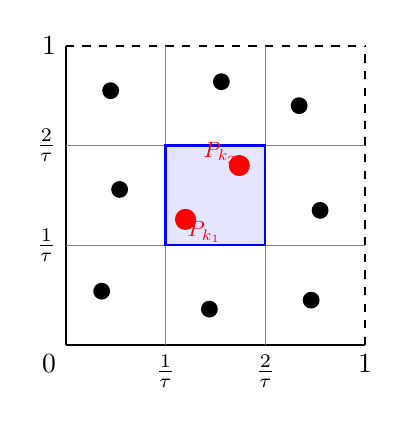
\begin{tikzpicture}[scale=3.8]
        % Единичный квадрат [0, 1)^2 для случая n = 2, \tau = 3
        \draw[thick] (0, 0) -- (1, 0);
        \draw[thick] (0, 0) -- (0, 1);
        \draw[thick, dashed] (1, 0) -- (1, 1);
        \draw[thick, dashed] (0, 1) -- (1, 1);

        % Сетка разбиения на \tau^2 = 9 малых квадратов со стороной 1/\tau
        \draw[gray, thin] (0.333, 0) -- (0.333, 1);
        \draw[gray, thin] (0.667, 0) -- (0.667, 1);
        \draw[gray, thin] (0, 0.333) -- (1, 0.333);
        \draw[gray, thin] (0, 0.667) -- (1, 0.667);

        % Выделенный малый квадрат с двумя точками P_{k_1} и P_{k_2}
        \fill[blue!10] (0.333, 0.333) rectangle (0.667, 0.667);
        \draw[blue, thick] (0.333, 0.333) rectangle (0.667, 0.667);

        % Точки P_k в различных ячейках
        \fill (0.12, 0.18) circle (0.8pt);
        \fill (0.82, 0.15) circle (0.8pt);
        \fill (0.15, 0.85) circle (0.8pt);
        \fill (0.78, 0.80) circle (0.8pt);
        \fill (0.48, 0.12) circle (0.8pt);
        \fill (0.18, 0.52) circle (0.8pt);
        \fill (0.85, 0.45) circle (0.8pt);
        \fill (0.52, 0.88) circle (0.8pt);

        % Две точки в одной ячейке
        \fill[red] (0.40, 0.42) circle (1pt) 
            node[below right=-2pt, scale=0.8] {$P_{k_1}$};
        \fill[red] (0.58, 0.60) circle (1pt) 
            node[above left=-2pt, scale=0.8] {$P_{k_2}$};

        % Подписи осей и размеров
        \node[below left] at (0, 0) {$0$};
        \node[below] at (0.333, 0) {$\frac{1}{\tau}$};
        \node[below] at (0.667, 0) {$\frac{2}{\tau}$};
        \node[below] at (1, 0) {$1$};
        \node[left] at (0, 0.333) {$\frac{1}{\tau}$};
        \node[left] at (0, 0.667) {$\frac{2}{\tau}$};
        \node[left] at (0, 1) {$1$};
    \end{tikzpicture}
    \caption{Разбиение единичного куба $[0, 1)^n$ при $n = 2$, $\tau = 3$ 
    на $\tau^n = 9$ ячеек со стороной $1/\tau$: среди $\tau^n + 1 = 10$ 
    точек две точки $P_{k_1}$ и $P_{k_2}$ попадают в одну ячейку.}
\end{figure}

\subsection{Комбинаторные задачи на подсчёт конфигураций}

\begin{problem}[\textbf{Чтение слова «КОМБИНАТОРИКА» в таблице}]
    В прямоугольной таблице записаны буквы слова «КОМБИНАТОРИКА» так, что 
    в левом верхнем углу стоит буква «К», а в каждой следующей строке слово 
    сдвигается на одну букву влево (образуя диагональные слои одинаковых 
    букв). Сколькими способами можно прочитать слово «КОМБИНАТОРИКА», 
    начиная с левой верхней буквы «К» и двигаясь на каждом шаге только 
    на одну клетку вправо или на одну клетку вниз?
\end{problem}

\begin{proof}[Решение]~\\
    \begin{quote}
        Слово «КОМБИНАТОРИКА» состоит из $L = 13$ букв. При заданном 
        заполнении таблицы клетка с координатами $(i, j)$ (где 
        $i \ge 0$ --- номер строки, $j \ge 0$ --- номер столбца) содержит 
        $(i + j + 1)$-ю букву слова «КОМБИНАТОРИКА».

        \begin{figure}[H]
            \centering
            \begin{tikzpicture}[scale=0.65]
                % Сетка первых букв таблицы слова КОМБИНАТОРИКА
                \node at (0, 4) {К}; \node at (1, 4) {О}; 
                \node at (2, 4) {М}; \node at (3, 4) {Б}; 
                \node at (4, 4) {И}; \node at (5, 4) {$\dots$}; 
                \node at (6.2, 4) {А};

                \node at (0, 3) {О}; \node at (1, 3) {М}; 
                \node at (2, 3) {Б}; \node at (3, 3) {И}; 
                \node at (4, 3) {Н}; \node at (5, 3) {$\dots$};

                \node at (0, 2) {М}; \node at (1, 2) {Б}; 
                \node at (2, 2) {И}; \node at (3, 2) {Н}; 
                \node at (4, 2) {А}; \node at (5, 2) {$\dots$};

                \node at (0, 1) {Б}; \node at (1, 1) {И}; 
                \node at (2, 1) {Н}; \node at (3, 1) {А}; 
                \node at (4, 1) {$\dots$};

                \node at (0, 0) {$\vdots$}; \node at (0, -0.8) {А};

                % Стрелки выбора направления из начальной клетки
                \draw[->, blue, thick] (0.3, 4) -- (0.7, 4);
                \draw[->, blue, thick] (0, 3.7) -- (0, 3.3);
                \draw[->, red, thick] (1.3, 4) -- (1.7, 4);
                \draw[->, red, thick] (1, 3.7) -- (1, 3.3);
            \end{tikzpicture}
            \caption{Фрагмент буквенной таблицы: из каждой текущей буквы 
            ведут ровно два допустимых шага (вправо или вниз) к следующей 
            букве слова.}
        \end{figure}

        Начиная движение из клетки $(0, 0)$ с первой буквой «К», для 
        перехода к каждой следующей из $12$ оставшихся букв слова мы на 
        каждом шаге имеем ровно $2$ независимых варианта хода: пойти на 
        одну клетку \textbf{вправо} или на одну клетку \textbf{вниз} (оба 
        хода увеличивают сумму координат $i + j$ на $1$ и приводят на 
        следующую по порядку букву слова).

        Таким образом, любой допустимый путь однозначно кодируется 
        последовательностью из $13 - 1 = 12$ команд из алфавита 
        $\{\text{Вправо}, \text{Вниз}\}$. По правилу умножения общее число 
        способов прочитать слово равно:
        \begin{equation} \label{eq:comb_paths}
            N = \underbrace{2 \cdot 2 \cdot \dots \cdot 2}_{12 \text{ раз}} = 
            2^{12} = 4096. \tag{7}
        \end{equation}
        \textbf{Ответ:} $2^{12} = 4096$ способов.
    \end{quote}
\end{proof}

\begin{problem}[\textbf{Задача об ожерельях и хороводах}]
    Сколькими способами можно составить замкнутое ожерелье из $n$ попарно 
    различных бусин ($n \ge 3$):
    \begin{enumerate}
        \item если ожерелье нельзя переворачивать в пространстве 
        (учитываются только циклические повороты в плоскости, как при 
        рассадке за круглым столом);
        \item если ожерелье можно свободно переворачивать в пространстве?
    \end{enumerate}
\end{problem}

\begin{proof}[Решение]~\\
    \begin{quote}
        Воспользуемся методом факторизации множества всех линейных 
        перестановок по отношению эквивалентности.

        \textbf{1. Учёт только вращений в плоскости (циклические 
        перестановки):}\\
        В ряд $n$ различных бусин можно выложить $n!$ способами. При 
        замыкании ряда в кольцо каждые $n$ линейных перестановок, 
        получающихся друг из друга циклическим сдвигом на 
        $0, 1, \dots, n - 1$ позиций по часовой стрелке, образуют одно и 
        то же ожерелье (один класс эквивалентности мощности $n$). 
        Следовательно, число различных циклических расположений равно:
        \begin{equation} \label{eq:circ_perm}
            N_{\text{круг}} = \frac{n!}{n} = (n - 1)!. \tag{8}
        \end{equation}
        Иначе это можно обосновать так: зафиксируем положение первой бусины 
        (чтобы устранить вращения), тогда оставшиеся $n - 1$ бусин можно 
        переставить относительно неё $(n - 1)!$ способами.

        \textbf{2. Учёт вращений и переворотов в пространстве:}\\
        Если ожерелье можно переворачивать (зеркально отражать), то 
        каждое ожерелье склеивается со своим зеркальным образом (обход 
        бусин по часовой стрелке переходит в такой же обход против часовой 
        стрелки). При $n \ge 3$ все бусины различны, поэтому ни одно 
        ожерелье не совпадает со своим перевёрнутым вариантом при простом 
        повороте. Каждый класс эквивалентности теперь содержит по $2$ 
        ориентации, откуда общее число ожерелий равно:
        \begin{equation} \label{eq:necklace_count}
            N_{\text{ожер}} = \frac{(n - 1)!}{2}. \tag{9}
        \end{equation}
    \end{quote}
\end{proof}

\begin{problem}[\textbf{Строго возрастающие целочисленные последовательности}]
    Сколько существует строго возрастающих конечных последовательностей 
    целых чисел, у которых первый и последний элементы зафиксированы и 
    равны соответственно:
    \begin{enumerate}
        \item начальный элемент равен $1$, а конечный равен $7$;
        \item начальный элемент равен $4$, а конечный равен $16$;
        \item начальный элемент равен $k$, а конечный равен $m + k$ 
        (где $k \in \Z$, $m \in \N$)?
    \end{enumerate}
\end{problem}

\begin{proof}[Решение]~\\
    \begin{quote}
        Решим задачу сразу в общем виде (пункт 3), когда строго 
        возрастающая последовательность целых чисел 
        $k = a_1 < a_2 < \dots < a_s = m + k$ начинается с числа $k$ и 
        заканчивается числом $m + k$.

        Заметим, что любое подмножество промежуточных целых чисел из 
        интервала $(k, m + k) \cap \Z = \{k + 1, k + 2, \dots, m + k - 1\}$ 
        после выбора однозначно выстраивается в порядке строгого 
        возрастания! Всего между числами $k$ и $m + k$ строго внутри 
        интервала лежат ровно:
        \[
            (m + k - 1) - (k + 1) + 1 = m - 1 \text{ целых чисел.}
        \]
        Каждое из этих $m - 1$ промежуточных чисел мы можем независимо 
        либо \textbf{включить} в нашу последовательность, либо 
        \textbf{не включать} (а крайние элементы $k$ и $m + k$ включены 
        обязательно). Следовательно, существует взаимно однозначное 
        соответствие (биекция) между искомыми строго возрастающими 
        последовательностями и всеми подмножествами $(m - 1)$-элементного 
        множества $\{k + 1, \dots, m + k - 1\}$.

        По формуле мощности булеана (или по биному Ньютона 
        $\sum_{j=0}^{m-1} C_{m-1}^j = 2^{m-1}$) получаем ответы для всех 
        трёх пунктов:
        \begin{enumerate}
            \item От $1$ до $7$: здесь $k = 1$, $m = 7 - 1 = 6$ 
            (промежуточные числа $\{2, 3, 4, 5, 6\}$ --- всего $5$ чисел). 
            Количество последовательностей равно $2^{6-1} = 2^5 = 32$.
            \item От $4$ до $16$: здесь $k = 4$, $m = 16 - 4 = 12$ 
            (промежуточные числа $\{5, 6, \dots, 15\}$ --- всего $11$ чисел). 
            Количество последовательностей равно $2^{12-1} = 2^{11} = 2048$.
            \item От $k$ до $m + k$: разность краёв равна $(m + k) - k = m$, 
            промежуточных чисел $m - 1$, поэтому количество строго 
            возрастающих последовательностей равно $2^{m-1}$.
        \end{enumerate}
    \end{quote}
\end{proof}

\subsection{Сочетания и число решений линейных уравнений}

\begin{proposition}[\textbf{Формулы числа сочетаний}]
    Напомним базовые формулы для числа сочетаний из $n$ типов элементов 
    по $k$:
    \begin{itemize}
        \item \textdef{Сочетания без повторений:}
        \begin{equation} \label{eq:comb_no_rep_sem5}
            C_n^k = \binom{n}{k} = \frac{n!}{k!(n - k)!} \tag{10}
        \end{equation}
        \item \textdef{Сочетания с повторениями} (число неотрицательных 
        целых решений уравнения $y_1 + y_2 + \dots + y_n = K$):
        \begin{equation} \label{eq:comb_rep_sem5}
            \bar{C}_n^K = C_{n+K-1}^K = C_{n+K-1}^{n-1} \tag{11}
        \end{equation}
    \end{itemize}
\end{proposition}

\begin{problem}
    Сколько целочисленных (натуральных) решений $(x_1, x_2, \dots, x_n)$ 
    имеет линейное уравнение:
    \begin{equation} \label{eq:eq_nat_sol}
        x_1 + x_2 + \dots + x_n = k \tag{12}
    \end{equation}
    при условии, что каждая неизвестная строго больше заданного целого 
    неотрицательного числа $m$: $\forall i = \overline{1, n} : x_i > m$?
\end{problem}

\begin{proof}[Решение]~\\
    \begin{quote}
        Поскольку $x_i$ и $m$ --- целые числа, строгое неравенство 
        $x_i > m$ равносильно нестрогому неравенству $x_i \ge m + 1$.

        Сведём задачу к классической схеме «шаров и перегородок» (сочетаниям 
        с повторениями) путём замены переменных. Для каждого 
        $i = \overline{1, n}$ введём новую неотрицательную целую переменную:
        \[
            y_i = x_i - (m + 1) \ge 0 \iff x_i = y_i + m + 1.
        \]
        Комбинаторно эта замена означает, что мы заранее кладём в каждый из 
        $n$ ящиков обязательный минимум по $m + 1$ шару (всего 
        $n(m + 1)$ шаров). Подставим выражение для $x_i$ в исходное 
        уравнение \eqref{eq:eq_nat_sol}:
        \begin{align*}
            (y_1 + m + 1) + (y_2 + m + 1) + \dots + (y_n + m + 1) &= k \\
            \iff y_1 + y_2 + \dots + y_n &= k - n(m + 1).
        \end{align*}
        Обозначим остаток распределяемых единиц через 
        $K = k - n(m + 1) = k - n m - n$.
        \begin{itemize}
            \item Если $k < n(m + 1)$, то $K < 0$, и уравнение 
            \eqref{eq:eq_nat_sol} не имеет ни одного решения в области 
            $x_i > m$ (ответ: $0$).
            \item Если $k \ge n(m + 1)$, то число неотрицательных целых 
            решений $(y_1, \dots, y_n) \in (\Z_{\ge 0})^n$ по формуле 
            сочетаний с повторениями \eqref{eq:comb_rep_sem5} равно:
            \[
                N = \bar{C}_n^{k - n(m + 1)} = 
                C_{n + k - n(m + 1) - 1}^{n - 1} = 
                C_{k - n m - 1}^{n - 1} = 
                \binom{k - n m - 1}{n - 1}.
            \]
        \end{itemize}
        В частном случае при $m = 0$ (классическая задача о числе 
        натуральных решений $x_i \ge 1$) формула даёт известный результат 
        $C_{k-1}^{n-1}$.
    \end{quote}
\end{proof}